\begin{question}[topic=gsm,type=exam,tags={20151014}]
\textbf{Hinweis:} In der Original Angabe ist die x-Achse des Diagramms nicht sichtbar, die Skalen auf der x-Achse sind somit geschätzt und es können unerwartete Ergebnisse auftreten.\\
Eine kompensierte \textbf{Nebenschluss-Gleichstrommaschine} hat folgende Daten. Eine Leerlaufkennlinie $U_i=f(I_E)$ bei $n=800~U/min$ ist gegeben (siehe Abb.\ref{fig:20151014}).\\
\begin{tabular}{L{2cm}l}
$I_{A,N}$ \dotfill &$300~A$\\
$U_{A,N}$ \dotfill & $250~V$ \\
$n_N$ \dotfill & $1000~\frac{U}{min}$
\end{tabular}
\begin{enumerate}
\item Skizzieren Sie die Schaltung der Nebenschlussmaschine am Gleichspannungsnetz. (\addpoints{1})
\item Wie groß ist die Spannungskonstante $k_1 \phi_N$ im Nennpunkt, das Nennmoment $M_N$ und die mechanische Nennleistung $P_N$ der Gleichstrommaschine, wenn ein Erregerwiderstand $R_E=15,6~\Omega$ verwendet wird? (\addpoints{3})
\item Wie groß ist dabei die Leerlaufdrehzahl $n_0$ und der Ankerwiderstand $R_A$ (\addpoints{2})
\item Berechnen Sie den Wirkungsgrad $\eta_N$ im Nennpunkt der Maschine unter Berücksichtigung des Ankerwiderstand $R_A$ und des Erregerwiderstands $R_E = 15,6~\Omega$. Die mechanischen Verluste, Bürstenverluste und Eisenverluste werden vernachlässigt. (\addpoints{1})
\item Die Maschine wird bei einer konstanten Drehzahl $n=800~U/min$ als Generator mit $R_E =15,6~\Omega$ eingesetzt und mit einem umschaltbaren Lastwiderstand $R_L = 0,1\, /\, 0,5\, /\, 1 ~\Omega$ belastet. Berechnen und Skizzieren Sie die (äussere) Generatorkennlinie $U_A=f(I_L)$ für die unterschiedlichen Belastungen inklusive Leerlauf des Generators mit $I_L = 0~A$. (\addpoints{3})
\end{enumerate}
\begin{figure}[H]
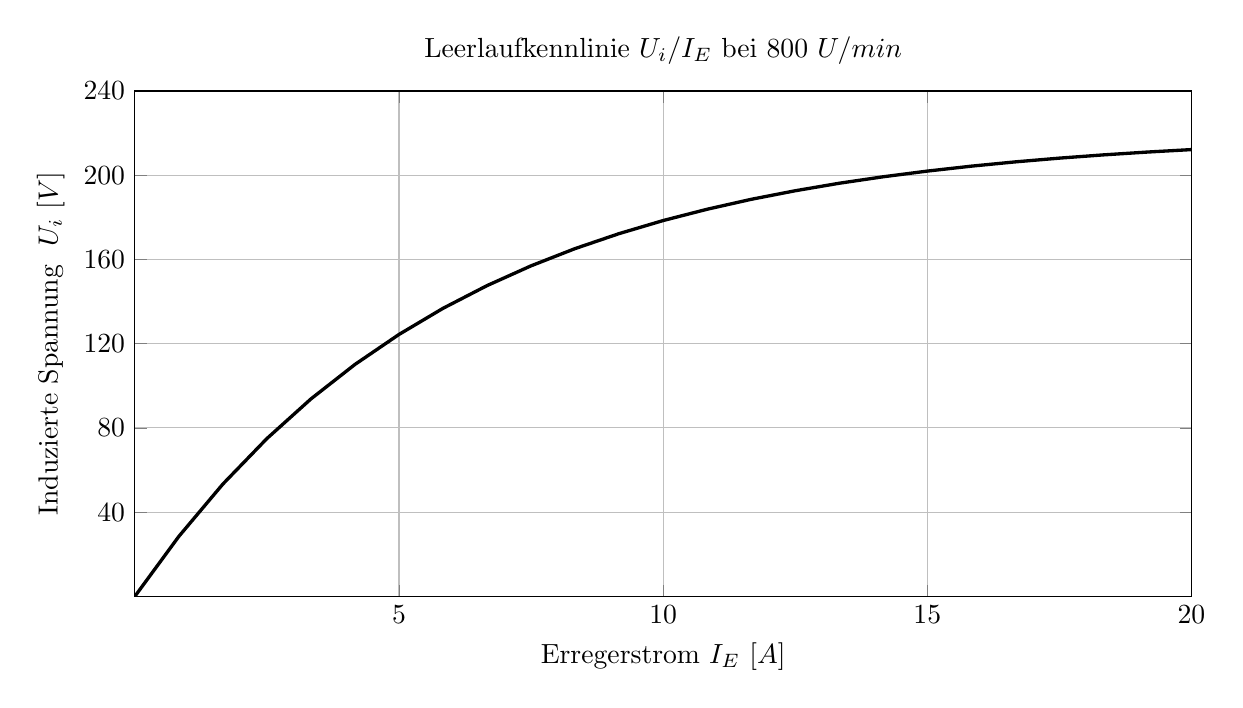
\begin{tikzpicture}
\begin{axis}[title={{Leerlaufkennlinie} $U_i/I_E$ {bei} $800 ~U/min$},xlabel={{Erregerstrom }$I_E \, \left[A\right]$ }, ylabel={{Induzierte Spannung } $U_i \, \left [V\right]$},
xtick= {5,10,15,20},width=15cm,height=8cm,
xmin = 0,xmax = 20,
ytick= {40,80,120,160,200,240},
ymin = 0 , ymax = 240,grid=major]
\addplot+
[id=exp,color=black,mark=none,domain=0:20, very thick]{220*(1-exp(-x/6))};
\end{axis}
\end{tikzpicture}
\caption{Leerlaufkennlinie} \label{fig:20151014}
\end{figure}
\end{question}
\begin{solution}
\begin{enumerate}
\item TikZ Grafik f\"ur Nebenschlussmaschine.
\item \textbf{Hinweis:} In der Original Angabe ist die x-Achse des Diagramms nicht sichtbar, die Skalen auf der x-Achse sind somit geschätzt und es k\"onnen unerwartete Ergebnisse auftreten.
\end{enumerate}
\end{solution}